% Created 2021-10-05 Tue 18:15
% Intended LaTeX compiler: pdflatex
\documentclass[journal=accacs,manuscript=article, email=true, layout=traditional]{achemso}
  \setkeys{acs}{biblabel=brackets,super=true,articletitle=False,maxauthors=0}
\usepackage[utf8]{inputenc}
\usepackage[T1]{fontenc}
\usepackage{fixltx2e}
\usepackage{url}
\usepackage{siunitx}
\usepackage{mhchem}
\usepackage{graphicx}
\usepackage{color}
\usepackage{amsmath}
\usepackage{textcomp}
\usepackage{wasysym}
\usepackage{latexsym}
\usepackage{amssymb}
\usepackage{minted}
\usepackage[section]{placeins}
\usepackage[linktocpage, pdfstartview=FitH, colorlinks=true, linkcolor=blue, anchorcolor=blue, citecolor=blue, filecolor=blue, menucolor=blue, urlcolor=blue]{hyperref}
\usepackage{attachfile}
\newcommand{\red}[1]{\textcolor{red}{#1}}
\newcommand{\blue}[1]{\textcolor{blue}{#1}}
\keywords{}
\renewcommand{\thefigure}{\arabic{figure}}
\renewcommand{\thetable}{\arabic{table}}
\usepackage{lmodern}
\usepackage{cleveref}
\author{Craig Waitt}
\affiliation{Department of Chemistry and Biochemistry, University of Notre Dame, Notre Dame, Indiana 46556, United States}
\author{Xuyao Gao}
\affiliation{Department of Chemical and Biomolecular Engineering, University of Notre Dame, Notre Dame, Indiana 4656, United States}
\author{William F. Schneider}
\email{wschneider@nd.edu}
\affiliation{Department of Chemical and Biomolecular Engineering, University of Notre Dame, Notre Dame, Indiana 46556, United States}
\alsoaffiliation{Department of Chemistry and Biochemistry, University of Notre Dame, Notre Dame, Indiana 46556, United States}
\date{}
\title{Orientational Flexibility of Organic Structure Directing Agents in CHA and AEI}
\begin{document}

\begin{header}
\end{header}

\newpage

\section{Workflow}
\label{sec:org52d8da7}
\subsection{Motivations}
\label{sec:org007409c}
\begin{enumerate}
\item OSDA/FW IE has been used as a reporter of an OSDAs crystallization affinity for a particular FW
\item While OSDA will ``fit'', some floppiness and even orientation flexibility exist which can influence computed IE
\item We have two approaches to sample orientational flexibility and compute IE:
\begin{enumerate}
\item Asexual Genetic Algorithm (AGA):
\begin{enumerate}
\item Uses information based on previously computed structures (orientations) to search for minimum structures
\begin{enumerate}
\item Energies evaluated with DFT
\end{enumerate}
\end{enumerate}
\item Classical Molecular Dynamics (CMD):
\begin{enumerate}
\item Randomly insert OSDA into FW
\item Run Dynamics at high Temp (5000 K)
\item Bin orientations
\item Re-run dynamics at ``reasonable'' Temp (500 K) on binned orientations to search for available orientations
\begin{enumerate}
\item Energies evaluated with Drieding force field (as used in the literature when sampling OSDA orientation space)
\end{enumerate}
\end{enumerate}
\end{enumerate}
\end{enumerate}

\subsection{Objectives}
\label{sec:org3c4d1c4}

\begin{enumerate}
\item Compare FW/IE interactions across two similar frameworks (CHA and AEI) across a family of OSDAs
\item Compare OSDA orientational flexibility
\item Compare strategies for extracting orientations and IE (mean IE in the CMD cases).
\item Compare predictive ability, dangers strategies.
\end{enumerate}

\subsection{Plan of Attack}
\label{sec:org7a4031c}

\begin{enumerate}
\item Craig will be doing the DFT/GA calculations in siliceous zeolites with CN OSDAs.
\begin{enumerate}
\item FWs are obtained from IZA (using IZA lattice constants)
\item A single OSDA is placed into one of the CHA and AEI cages
\begin{enumerate}
\item OSDA nitrogens are replaced with carbons to maintain charge neutrality
\end{enumerate}
\item An AGA is used to sample the configurational space the OSDA can adopt within a FW cage
\begin{enumerate}
\item 20 parents are randomly displace within a cage
\item The structures are minimized using the PBE-D3 functional
\begin{enumerate}
\item Resulting energies are used to score the candidates
\end{enumerate}
\item Parents used within the AGA are selected based on a Boltzmann distribution
\item Those parents undergo a mutation which translates and rotates them in the cage.
\item This process is repeated until 10 children have been generated
\item The children are minimized using the PBE-D3 functional and steps 3-6 are repeated until a total of 50 structures have been generated
\end{enumerate}
\item These 50 candidates are a representation of the global configurations an OSDA can adopt with a particular cage
\end{enumerate}
\end{enumerate}

\begin{figure}
\begin{center}

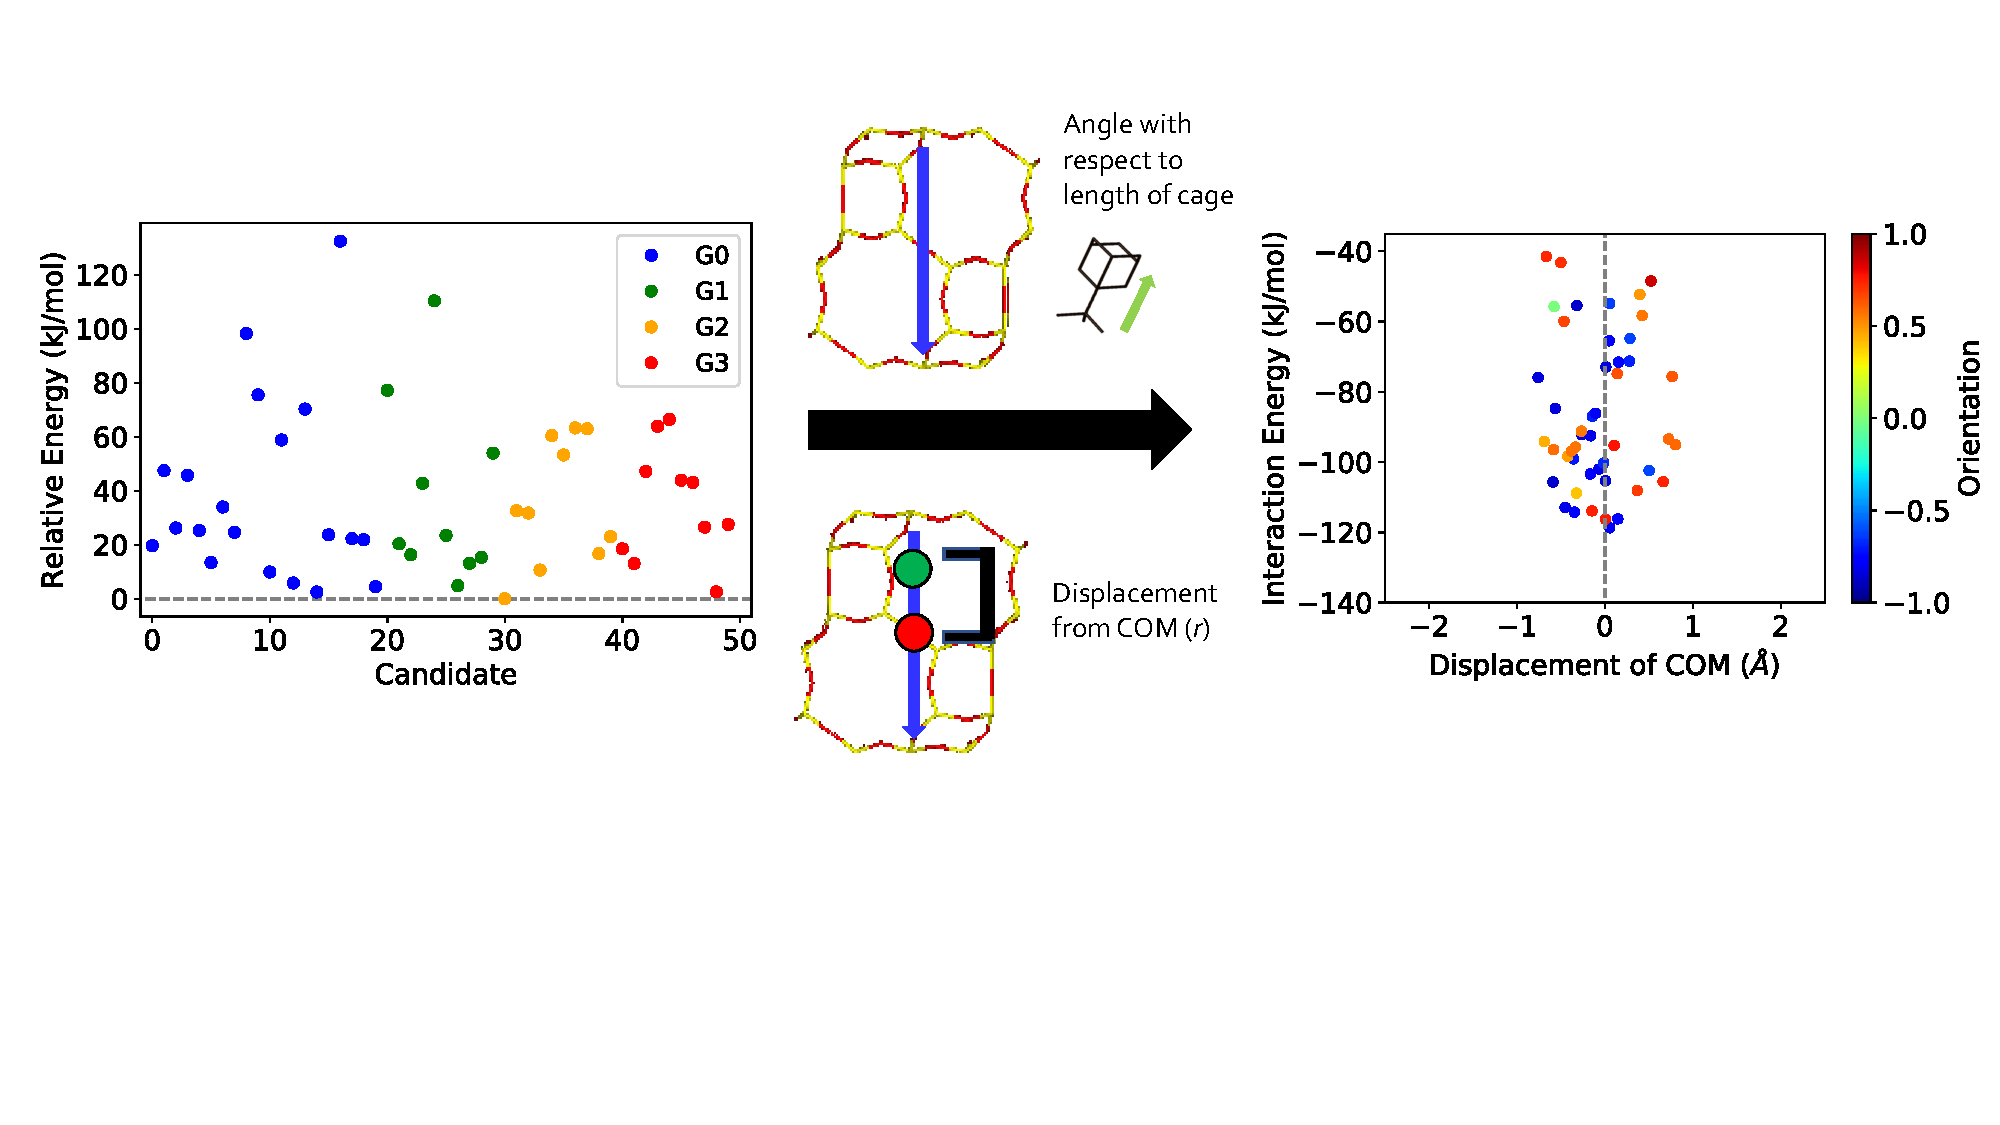
\includegraphics[scale=.5,trim={0cm 5cm 0cm 0cm},clip]{./Figures/DFT_GA_to_Ori.pdf}
\caption{Schematic representation of the DFT/AGA proceedure. Candidates are minimized are generated in sequencial step and minimized with the PBE-D3 functional. We select the tertiary carbon (previously the notrogen) of an OSDA and look at the orientation and translation within a framwork with respect to a vector which describes the length of the cage. The lowest energy point corresponds to the most favorable configuration the OSDA can sit within the framework and is denoted as $\text{IE}^{\text{DFT}}_{\text{L}}$}. 
\label{fig:DFT_GA_to_Ori} 

\end{center}
\end{figure}

\begin{enumerate}
\item Xuyao will be doing the CMD calculations in siliceous zeolites with CN OSDAs.
\end{enumerate}






\section{Results to Date}
\label{sec:org9931970}
\subsection{OSDAs of interest and the FW they crystallize}
\label{sec:org95c7882}
Using the parameters/models discussed above, we will first compare the lowest energy structure using GA and lowest energy average CMD energy to see if PBE and Dreiding predict similar or differenct affinities for OSDAs to crystallize CHA or AEI. The table below summarizes the OSDAs used in this study and is separated based on which OSDA crystallizes which framework. 

\begin{center}
\begin{tabular}{c|c}
\hline
Zeolite & OSDAs \\
\hline
CHA          & TMADA, DEDMP-3c, DEDMP-3t, TMBCN, PMCH-3c, PMCH-3t \\
AEI          & DMDMP-2c, DMDMP-3c, DMDMP-3t, DEDMP-2c, DMBCN \\
Intergrowth  & Tetra \\
\hline
\end{tabular}
\end{center}

The names for these OSDA's are abbreviations for there full names. We will need to think of a clever way on how to present each one (e.g. Template A,B,C etc.)

\subsection{Rigid Framework Assumption}
\label{sec:org04f7113}
Besides evaluating energy differences differently (Dreiding vs. DFT), there is one considerable difference between our two models. The CMD method is restricted to a rigid framework (since Si-O parameters are unknown for Drieding). Therefore it is a reasonable question to ask, ``What happens to the DFT results when the framework is rigid and relaxed?'' To answer this question, I did two set of DFT calculations. First, I performed my AGA by minimizing the OSDA/FW to a local minimum. I then searched for the lowest energy structure, took the initial structure file (which as the Si-O atoms in the zeolite from IZA) and reoptimized the structures but kept the zeolite fixed. This gives me two structures, one where only the OSDA was relaxed to a minimum and one where both the OSDA and Zeolite are relaxed to a minimum. The results for CHA are shown in the Figure below.

\begin{figure}
\begin{center}

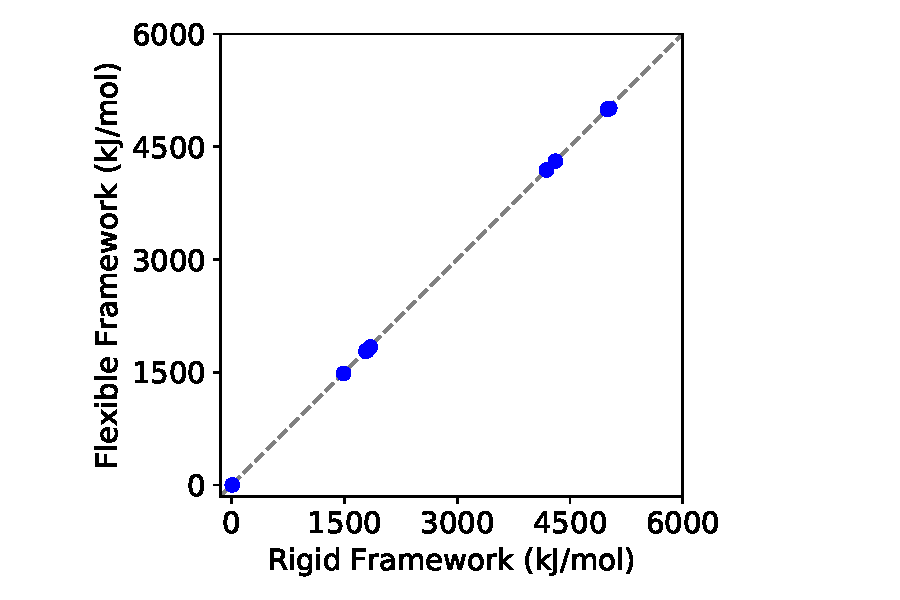
\includegraphics[scale=.5,trim={0cm 0cm 0cm 0cm},clip]{./Figures/Framework-flex.pdf}
\caption{Parity plot comparing the the lowest energy orientation of each OSDA from the GA (flexible framework), compared to a rigid framework. $R^{2}$ value of the data compared to the parity line is 0.99999. }. 
\label{fig:Rig_v_Flex} 

\end{center}
\end{figure}

Figure \ref{fig:Rig_v_Flex} compares the energy of the Rigid framework to the flexible framework. The largest deviation from the parity line is approximately 18 kJ/mol (DMDMP-2c in CHA). and the points lie on the parity line. As such it doesn't make too much of a difference if the framework is allowed to relax to a minimum. For the remainder of this study the framework is flexible.

\subsection{Orientation Freedom}
\label{sec:org4c19826}
We use both the AGA and MD sampling to compare the orientational freedom of an OSDA in a framework. We are comparing orientational space where the OSDA and FW are allowed to be relaxed (DFT/AGA) and ones where only the OSDA is allowed to move(CMD). We have evaluated all of the OSDAs in the table above (with the exception of one of the DMDMP isomers) and we are going to compare two sets of results in this outline. 

We have devised a scheme to visualize the orientation an OSDA adopts within the cage. We compute the angle the OSDA makes with the long axis with the cage (using the tertiary carbon and an adjacent carbon or the center of mass with respect to DMBCN which does not have an adjacent carbon), and the displacement of the tertiary carbon along that vertical vector. 

\begin{figure}
\begin{center}

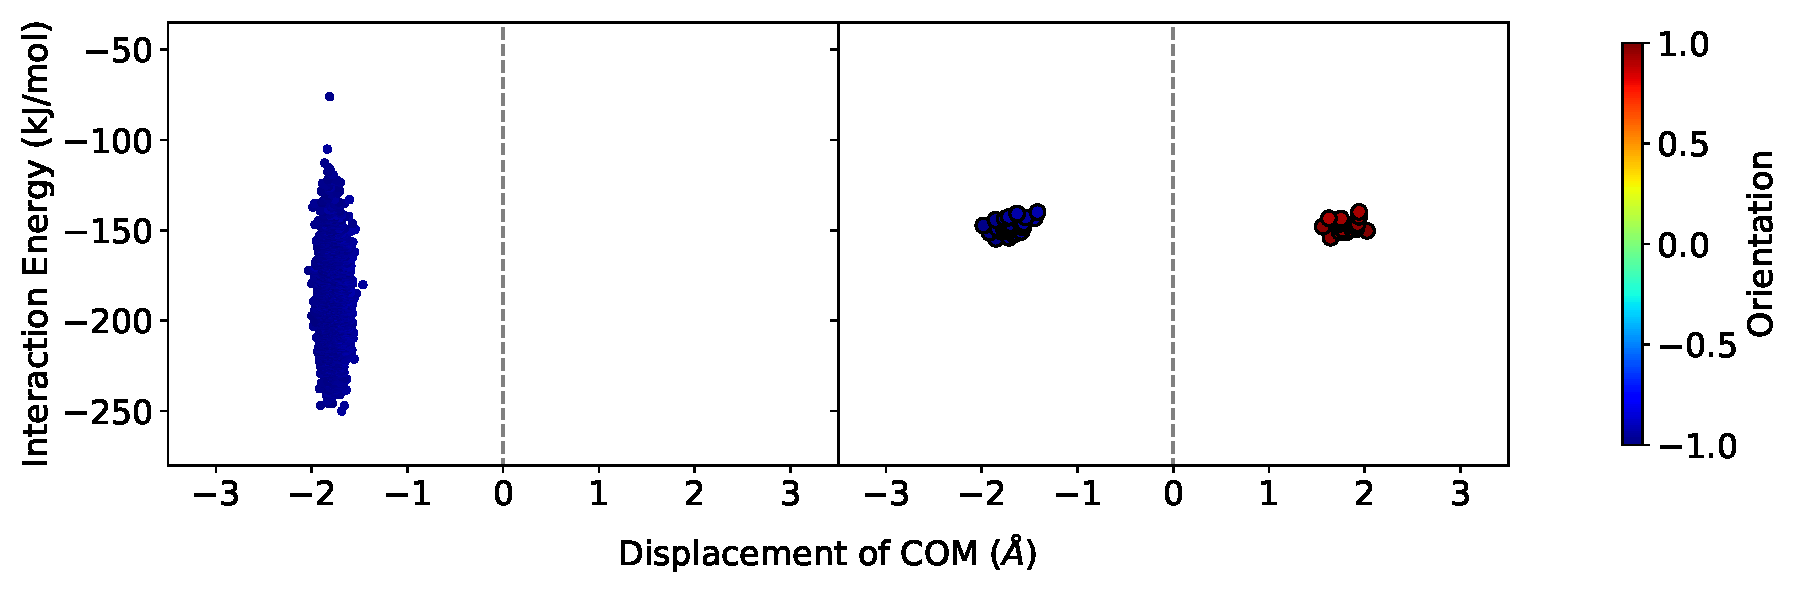
\includegraphics[scale=.5]{./Figures/CHA-GA-CMD-TMADA.pdf}
\caption{TMADA in CHA. Left CMD results, Right DFT/AGA results.} 
\label{fig:TMADA-CHA} 

\end{center}
\end{figure}

The results for fig \ref{fig:TMADA-CHA} above show that TMADA is fairly rigid in the CHA cage. There are two degenerate orientations of TMADA in CHA in the AGA results, a downward and upward orientation (blue and red points respectively). These are degenerate given the symmetry of the CHA cage. The CMD results only predict one orientation however. The energy barrier to flip to another orientation is greater than 5000 K and thus the CMD sampling method did not sample the other regime. Otherwise, Comparison of the two blue points is fairly similar. The lowest energy structure from DFT is about 30 kJ/mol higher in energy than the average CMD energy. For other OSDA's in CHA, there is a mixture of results that look like the figure above (where some regime is missed, due to the high barrier to rotate) and others where the CMD and GA results look ``identical.''

\begin{figure}
\begin{center}

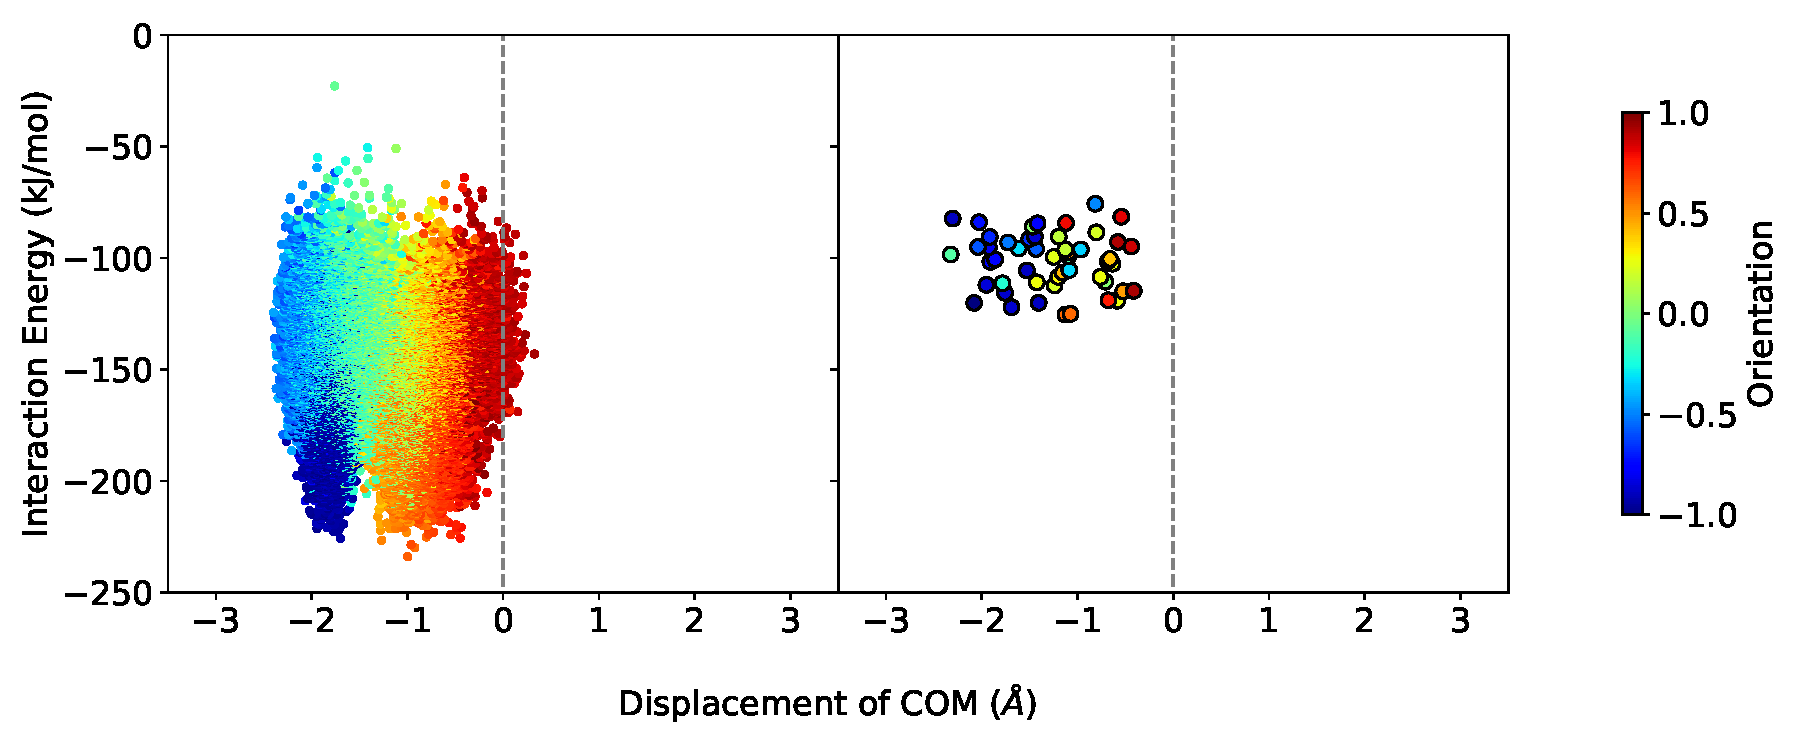
\includegraphics[scale=.5]{./Figures/AEI-GA-CMD-DMDMP_2c.pdf}
\caption{DMDMP-2c in CHA. Left CMD results, Right DFT/AGA results.} 
\label{fig:DMDMP-2c-AEI} 

\end{center}
\end{figure}

The results for fig \ref{fig:DMDMP-2c-AEI} are for DMDMP-2c in AEI. Both the left and right figures look very similar. The AEI wide frame of the cage is sufficiently large enough for the collection of OSDAs to rotate and change orientations within the cage. Both techniques produce similar orientational flexibility. DMDMP-2c fits fairly loose within the cage, as do the majority of OSDAs for this study. The lowest energy orientation from the DFT results is at about 0.5 and has an energy of -125 kJ/mol, and the CMD results of the same orientation have an energy of approximately 50 kJ/mol higher in energy than the average CMD results for that orientation. 

\subsection{Dreiding vs. DFT}
\label{sec:org3c36611}
We can compare the overall similarity of the Dreiding and DFT predicted energies for the lowest energy average configuration and lowest energy structure respectively. The Figure bellow plot a parity plot between the two. There is something not quiet right.
\end{document}